\documentclass{beamer}

\usepackage[utf8]{inputenc}
\usepackage[T1]{fontenc}
\usepackage[ngerman]{babel}
\usepackage{lmodern}
\usepackage{amsmath}
\usepackage{listings}
\usepackage{xcolor}

%%% Choose theme
% \usetheme{Montpellier} 
% \usecolortheme{beaver}
\usetheme{Madrid} 
\usecolortheme{seahorse}
\beamertemplatenavigationsymbolsempty

% Syntax higlighting colors
\definecolor{mygreen}{rgb}{0,0.6,0}
\definecolor{mygray}{rgb}{0.5,0.5,0.5}
\definecolor{mymauve}{rgb}{0.58,0,0.82}
\lstset{
  numbers = left,
  xleftmargin = 2em,
  tabsize = 4,
  backgroundcolor=\color{white},   % choose the background color
  basicstyle=\fontsize{9}{9}\ttfamily,        % size of fonts used for the code
  breaklines=true,                 % automatic line breaking only at whitespace
  % captionpos=b,                    % sets the caption-position to bottom
  commentstyle=\itshape\color{mygray},    % comment style
  escapeinside={\%*}{*)},          % if you want to add LaTeX within your code
  keywordstyle=\bfseries\color{blue},       % keyword style
  stringstyle=\color{mymauve},     % string literal style
  moredelim=**[is][\color{red}]{@}{@}  % emphazise @word@ with color
}

\title{ROS Unit Tests Workshop}
\author{Lukas Hoyer}
\institute[]{Otto-von-Guericke-Universität Magdeburg}
\date{12.06.2017}

\begin{document}
\maketitle

\begin{frame}{Softwareentwicklung}
	\begin{block}{Spezifikation}
		= Beschreibung des geforderten Systems
		\begin{itemize}
			\item Was soll von einem System geleistet werden?
			\item Was sind die funktionalen und nicht-funktionalen Anforderungen?
		\end{itemize}
	\end{block}
	\begin{block}{Verifikation}
		= entspricht Software der Spezifikation	
		\begin{itemize}
			\item Arbeitet das Programm korrekt?
			\item Erfüllt das Programm die Anforderungen?
		\end{itemize}
	\end{block}
\end{frame}

\begin{frame}{Motivation: Ariane 5}
\begin{itemize}
	\item Übernahme von Hard- und Software für das
Trägheitsnavigationssystem (SRI) aus der Ariane 4
	\begin{itemize}
		\item SRI keine Überlaufkontrolle für bestimmte Variablen aufgrund der maximalen Beschleunigung der Ariane 4
		\item keine Aufnahme von Flugbahndaten der Ariane 5 in die Spezifikation des SRI	
	\end{itemize}
	\pause
	\item Ariane 5 höhere Beschleunigungen als Ariane 4 -> Überlauf
	\begin{itemize}
		\item Ausfall von zwei redundanten Modulen aufgrund gleicher Software
		\item Fehlercode wurde vom Onboard-Computer fälschlicherweise als Flugbahndaten interpretiert
		\item Falsche Korrektur der Flugbahn
		\item Selbstzerstörung
	\end{itemize}
	\pause
	\item 370 Mio. \$ Schaden
\end{itemize}
\end{frame}

\begin{frame}{Motivation: Ariane 5}
	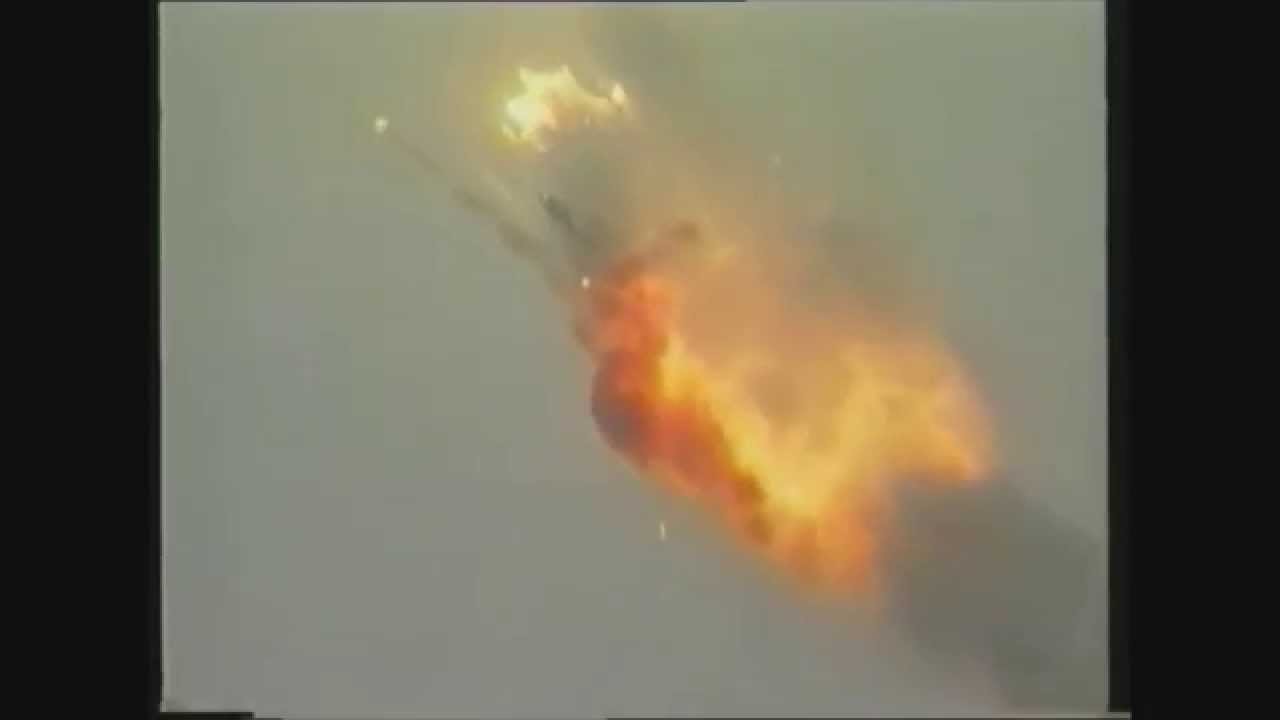
\includegraphics[width=\textwidth]{img/ariane5.jpg}

	\url{https://www.youtube.com/watch?v=A1gGGDG580E}
\end{frame}

\begin{frame}{Softwaretests}
	\begin{block}{Softwaretests}
		\begin{itemize}
			\item Ausführen eines Systems oder einer Komponente unter bestimmten Bedingungen
			\item Evaluierung bestimmter Aspekte des Systems bzw. der Komponente
			\item \text{''}Program testing can be used to show the presence of bugs, but never show their absence!\text{''} -- Dijkstra
		\end{itemize}
	\end{block}
	\pause
	\begin{block}{Unittest}
		\begin{itemize}
			\item Prüfung von funktionalen Einzelteilen (Units) auf korrekte Funktionalität
		\end{itemize}
	\end{block}
	\begin{block}{Integrationstest}
		\begin{itemize}
			\item Testen des Zusammenspiels voneinander abhängiger Komponenten eines Systems
		\end{itemize}
	\end{block}
\end{frame}

\begin{frame}{Unittests}
	\begin{block}{Vorteile von Unittests}
	\begin{itemize}
		\pause
		\item keine \text{''}Wegwerftests\text{''}
		\item Frühzeitiges Erkennen von Fehlern
		\item Gute Eingrenzung von Fehlern
		\item API-Dokumentation
		\item Refactoring überprüfen
		\item Verhindern von erneutem Auftreten eines Bugs
		\item Schneller als andere Testarten
		\item Design Hilfe
		\item Durch zwingende Vermeidung von Abhängigkeiten bleibt Quellcode modularer
	\end{itemize}
	\end{block}
\end{frame}

\begin{frame}[fragile]{Einrichten des Workspaces}
\begin{itemize}
\item Erstellen eines Workspaces
\begin{lstlisting}[language=bash]
mkdir -p ~/workshop_ws/src
cd ~/workshop_ws/src/
catkin_init_workspace
cd ~/workshop_ws && catkin_make
source devel/setup.bash #(temporary)
\end{lstlisting}
\pause
\item Neues Package anlegen
\begin{lstlisting}[language=bash]
cd ~/workshop_ws/src/
catkin_create_pkg ros_unit_tests_workshop roscpp
\end{lstlisting}
\item package.xml anpassen (Entwickler, Beschreibung, usw.)
\end{itemize}
\end{frame}

\begin{frame}[fragile]{Funktionalität}
\begin{itemize}
\item Quellcode unter: \url{https://github.com/lhoyer/ros_unit_tests_workshop/}
\item Hinzufügen my\_math.h
\begin{lstlisting}[language=c++]
#pragma once
class MyMath {
public:
	MyMath() {}
	int knobel(int x, int y);
protected:
	int mLastBase = 0;
	int nextSquare();
};
\end{lstlisting}
\end{itemize}
\end{frame}

\begin{frame}[fragile]{Funktionalität}
\begin{itemize}
\item Hinzufügen my\_math.cpp
\begin{lstlisting}[language=c++]
#include "my_math.h"
#include <stdexcept>
int MyMath::knobel(int x, int y) {
	if (x < 0 || y < 0) throw std::invalid_argument("received negative value");
	if (x == 0)
		return y;
	while (y != 0) {
		if (x > y) x = x -y;
		else y = y - x;
	}
	return x;
}
int MyMath::nextSquare() {
	int a=0, b=0, c=0;
	mLastBase++;
	while (a <= mLastBase) {
		a = a+1;
		b = a+a-1;
		c = b+c;
	}
	return c;
}
\end{lstlisting}
\end{itemize}
\end{frame}

\begin{frame}[fragile]{Funktionalität}
\begin{itemize}
\item Anpassen CMakeLists.txt
\begin{lstlisting}[language=make]
## Declare a C++ library
add_library(${PROJECT_NAME}
  src/my_math.cpp
)
## Add dependencies
add_dependencies(${PROJECT_NAME} ${${PROJECT_NAME}_EXPORTED_TARGETS} ${catkin_EXPORTED_TARGETS})
## Specify libraries to link a library or executable target against
target_link_libraries(${PROJECT_NAME}
  ${catkin_LIBRARIES}
)
\end{lstlisting}
\end{itemize}
\end{frame}

\begin{frame}[fragile]{Einrichten von gtest unter ROS}
\begin{itemize}
\item Anpassen CMakeLists.txt
\begin{lstlisting}[language=make]
# Compile as C++11, supported in ROS Kinetic and newer
add_compile_options(-std=c++11)
# ...
include_directories(
  ${catkin_INCLUDE_DIRS}
  src/
)
# ...
# Add gtest based cpp test target and link libraries
catkin_add_gtest(${PROJECT_NAME}-test test/mytest.cpp)
if(TARGET ${PROJECT_NAME}-test)
  target_link_libraries(${PROJECT_NAME}-test ${PROJECT_NAME})
endif()
\end{lstlisting}
\end{itemize}
\end{frame}

\begin{frame}[fragile]{GTest Frame}
test/mytest.cpp:
\begin{lstlisting}[language=c++]
#include <ros/ros.h>
#include <gtest/gtest.h>
#include <thread>
#include "my_math.h"

// Here you can add your test cases

int main(int argc, char** argv){
    ros::init(argc, argv, "MyTestNode");
    testing::InitGoogleTest(&argc, argv);
    ros::NodeHandle roshandle;
    std::thread t([]{while(ros::ok()) ros::spin();});
    if( ros::console::set_logger_level(ROSCONSOLE_DEFAULT_NAME, 
    	ros::console::levels::Info) ) {
       ros::console::notifyLoggerLevelsChanged();
    }
    // ::testing::GTEST_FLAG(filter) = "MyTest.knobelTest";
    auto res = RUN_ALL_TESTS();
    ros::shutdown();
    return res;
}
\end{lstlisting}
\end{frame}

\begin{frame}{GTest Frame wichtige Funktionen}
\begin{description}
	\item[InitGoogleTest(...)]: Aufsetzen der Testumgebung
	\item[set\_logger\_level(...)]: Setzen des Loggerlevels für die Tests (Debug, Info, Warn, Error, Fatal), ab dem Meldungen angezeigt werden
	\item[GTEST\_FLAG(filter) = \text{''}Suite.Test\text{''}]: Nur einen bestimmten Test Case ausführen
	\item[RUN\_All\_TESTS()]: Ausführen aller Test Cases
\end{description}
\end{frame}

\begin{frame}[fragile]{Beispiel Test Case}
\begin{lstlisting}[language=c++]
TEST(MyTest, knobelTest) {
    MyMath mymath;
    EXPECT_EQ(1, mymath.knobel(7,13)) << "gcd(7,13)=1";
    ASSERT_EQ(27, mymath.knobel(27,27)) << "gcd(27,27)=27";
    EXPECT_EQ(6, mymath.knobel(12,18)) << "gcd(12,18)=6";
    EXPECT_EQ(5, mymath.knobel(5,0)) << "gcd(5,0)=5";
    EXPECT_THROW(mymath.knobel(12,-18), std::invalid_argument) << "Our gcd isn't defined for negative values";
}
\end{lstlisting}
\pause
\begin{description}
	\item[TEST(Suite, Test)]: Test Case mit Namen \textit{Test} in Test Suite \textit{Suite}
	\item[EXPECT\_EQ(expected, value)]: Prüfen, ob Werte gleich sind
	\item[ASSERT\_EQ(expected, value)]: Prüfen, ob Werte gleich sind; bei Fehlschlag Abbruch des Tests
	\item[...\_NE()]: Prüfen, ob Werte unterschiedlich sind
	\item[...\_LT()]: Prüfen, ob erster Wert <= zweiter Wert
	\item[...\_FALSE()]: Prüfen, ob Wert false ist
	\item[...\_STREQ()]: Prüfen, ob Strings gleich sind
\end{description}
\end{frame}

\begin{frame}[fragile]{Test Case ausführen}
\begin{itemize}
\item Roscore starten
\begin{lstlisting}[language=bash, numbers=none]
roscore
\end{lstlisting}
\item Alle Test ausführen
\begin{lstlisting}[language=bash, numbers=none]
catkin_make run_tests
\end{lstlisting}
\item Nur Test des Pakets ausführen
\begin{lstlisting}[language=bash, numbers=none]
catkin_make run_tests_ros_unit_tests_workshop
\end{lstlisting}
\item Beispielausgabe eines Tests
\begin{lstlisting}[language=bash, numbers=none]
[==========] Running 1 test from 1 test case.
[----------] Global test environment set-up.
[----------] 1 test from MyTest
[ RUN      ] MyTest.knobelTest
[       OK ] MyTest.knobelTest (0 ms)
[----------] 1 test from MyTest (0 ms total)

[----------] Global test environment tear-down
[==========] 1 test from 1 test case ran.
[  PASSED  ] 1 test.
\end{lstlisting}
\end{itemize}
\end{frame}

\lstdefinestyle{using_colors}{
  moredelim=**[is][\color{red}]{@}{@},
}

\begin{frame}[fragile]{Fixtures}
\begin{Definition}
Ein Fixture ist eine Klasse, die als Umgebungsvorlage für die Ausführung eines Tests benutzt wird. 
\end{Definition}
\pause
\begin{lstlisting}[language=c++, style=using_colors]
class MyMathTestSuite : public @::testing::Test@, public MyMath {
public:
    MyMathTestSuite() {
    	mLastBase = 5;
    }
};

@TEST_F@(MyMathTestSuite, nextSquareTest) {
	EXPECT_EQ(5, mLastBase);
	EXPECT_EQ(36, nextSquare()) << "Square of 6 should be 36";
	EXPECT_EQ(6, mLastBase);
	EXPECT_EQ(49, nextSquare()) << "Square of 7 should be 49";
	EXPECT_EQ(7, mLastBase);
}
\end{lstlisting}
\end{frame}

\begin{frame}[fragile]{Was ist schiefgelaufen?}
Ausgabe:
\begin{lstlisting}[language=bash, numbers=none]
[ RUN      ] MyMathTestSuite.nextSquareTest
ros_unit_tests_workshop/test/mytest.cpp:24: Failure
Value of: nextSquare()
  Actual: 49
Expected: 36
ros_unit_tests_workshop/test/mytest.cpp:26: Failure
Value of: nextSquare()
  Actual: 64
Expected: 49
[  FAILED  ] MyMathTestSuite.nextSquareTest (0 ms)
\end{lstlisting}
\pause
Auflösung:
\begin{lstlisting}[language=c++, style=using_colors]
int MyMath::nextSquare() {
	int a=0, b=0, c=0;
	mLastBase++;
	while (a @<@ mLastBase) {
		a = a+1;
		b = a+a-1;
		c = b+c;
	}
	return c;
}
\end{lstlisting}
\end{frame}

\begin{frame}{Unittests}
	\begin{block}{Good Practices Unittests}
	\begin{itemize}
		\item Test Cases unabhängig voneinander
		\item Jede Funktionalität in separatem Test Case
		\item Ergebnisse testen, nicht Implementierung
		\item Überspezifizierung vermeiden
		\item Tests müssen deterministisch sein
		\item Tests müssen schnell sein
	\end{itemize}
	\end{block}
\end{frame}

\end{document}